\documentclass[ignorenonframetext,notheorems,aspectratio=1610]{beamer}
\usetheme[compress]{Madrid}
\usecolortheme{iwr}
\usepackage{../mathsim}
\mathtoolsset{showonlyrefs}
\excludecomment{solution}
\externaldocument{main}

\makeatletter
\def\BT@with[#1]#2(#3){\begin{block}{#3 \capitalizewords{#2} (#1)}}
\def\BT@without#1(#2){\begin{block}{#2 \capitalizewords{#1}}}
\def\endblocktheorem{\end{block}}
\makeatother
\def\mylabel#1{}
\let\label\mylabel
%\renewcommand{\label}[1]{}
\renewcommand{\eqref}[1]{(\ref{#1})}
\renewcommand{\define}[1]{\textbf{#1}}

\begin{document}
\frame{\tableofcontents}
\section{From elliptic to mixed problems}
\frame {\input {blocks/Notation-vector-diff-operators.tex}}
\frame {\input {blocks/Definition-strain-tensor.tex}}
\frame {\input {blocks/Definition-hooke.tex}}
\frame {\input {blocks/Definition-weak-lame-navier.tex}}
\frame {\input {blocks/Problem-frobenius.tex}}
\frame {\input {blocks/Assumption-korn-inequality.tex}
  \input {blocks/Lemma-korn.tex}}
\frame {\small\input {blocks/Problem-elasticity-standard.tex}}

\begin{frame}
  \frametitle{Example: hanging sheet}
  \centering
  \begin{tabular}{ccc}
    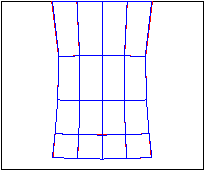
\includegraphics[width=.25\textwidth]{./graph/elasticity/stalactite-0}
    &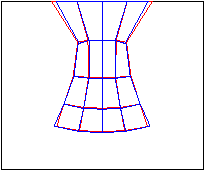
\includegraphics[width=.25\textwidth]{./graph/elasticity/stalactite-1}
    &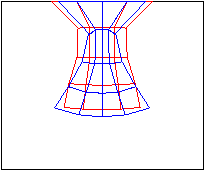
\includegraphics[width=.25\textwidth]{./graph/elasticity/stalactite-2}
    \\
    $\lambda = 1$&$\lambda = 10$&$\lambda = 100$
    \\\\
    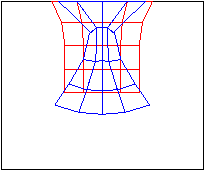
\includegraphics[width=.25\textwidth]{./graph/elasticity/stalactite-3}
    &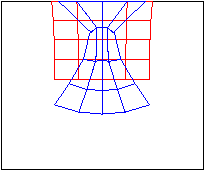
\includegraphics[width=.25\textwidth]{./graph/elasticity/stalactite-4}
    &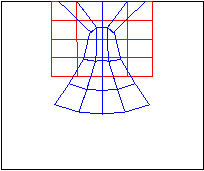
\includegraphics[width=.25\textwidth]{./graph/elasticity/stalactite-5}
    \\
    $\lambda = 1000$&$\lambda = 10000$&$\lambda = 100000$
  \end{tabular}
\end{frame}
\frame {\input {blocks/Definition-displacement-pressure.tex}}
\frame {\input {blocks/Definition-lame-navier-strong.tex}}
\frame {\input {blocks/Definition-saddle-point-operators.tex}}
\frame {\input {blocks/Definition-saddle-point-abstract.tex}}
\frame {\input {blocks/Notation-saddle-point-form.tex}}
\frame {\input {blocks/Definition-schur-complement.tex}
  \input {blocks/Lemma-schur-complement1.tex}}
\frame {\input {blocks/Lemma-schur-definiteness.tex}}
\frame {\input {blocks/Definition-stokes-eq1.tex}}
\frame {\input {blocks/Definition-solenoidal.tex}}
\frame {\input {blocks/Lemma-stokes-equivalence.tex}}
\frame {\input {blocks/Definition-stokes-eq2.tex}}
\frame {\input {blocks/Definition-stokes-boundary2.tex}}
\frame {\input {blocks/Lemma-divergence-compatibility.tex}
\input {blocks/Notation-pressure-constant.tex}}
\frame {\input {blocks/Theorem-minimization.tex}}
\frame {\input {blocks/Definition-reduced-problem.tex}
\input {blocks/Lemma-reduced-wellposedness.tex}}
\frame {\input {blocks/Theorem-lagrange-multiplier.tex}}
\frame {\input {blocks/Problem-lagrange-multiplier.tex}}
\frame {\input {blocks/Corollary-stokes-lagrange.tex}}

\section{Conditions for well-posedness}
\frame {\input {blocks/Problem-unbounded-inverse.tex}}
\frame {\input {blocks/Problem-lax-milgram-not-applicable.tex}}
\frame {\input {blocks/Theorem-la-invertible.tex}}
\frame {\input {blocks/Theorem-svd.tex}}
\frame {\input {blocks/Corollary-svd-order.tex}}
\frame {\input {blocks/Definition-ker-range-rn.tex}
\input {blocks/Definition-orthogonal1.tex}}
\frame {\input {blocks/Lemma-ker-coker-rn.tex}
\input {blocks/Corollary-ker-coker-iso.tex}
\input {blocks/Corollary-svd-infsup.tex}}
\frame {\input {blocks/Definition-infsup1.tex}
\input {blocks/Lemma-infsup2.tex}
\input {blocks/Problem-inf-sup-equivalence.tex}}
\frame {\input {blocks/Definition-polar-orthogonal.tex}
\input {blocks/Lemma-orthogonal-closed.tex}
\input {blocks/Theorem-orthogonal-complement.tex}}
\frame {\input {blocks/Definition-orthogonal-projection.tex}}
\frame {\input {blocks/Lemma-polar-orthogonal-hilbert.tex}}
\frame {\input {blocks/Theorem-closed-range.tex}}
\frame {\input {blocks/Theorem-open-mapping.tex}
\input {blocks/Lemma-closed-infsup.tex}}
\frame {\input {blocks/Theorem-infsup-well-equivalence.tex}}
\frame {\input {blocks/Corollary-infsup-well-posedness1.tex}}
\frame {\input {blocks/Theorem-infsup-well-posedness2.tex}}
\frame {\input {blocks/Theorem-infsup-mixed1.tex}}
\frame {\input {blocks/Theorem-infsup-mixed2.tex}}
\frame {\input {blocks/Problem-inhomogeneous-continuity.tex}}
\frame {\input {blocks/Assumption-mixed-elliptic.tex}}
\frame {\input {blocks/Definition-kerbh.tex}}
\frame {\input {blocks/Definition-mixed-galerkin.tex}}
\frame {\input {blocks/Theorem-galerkin-mixed-u-kerbh.tex}}
\frame {\input {blocks/Corollary-galerkin-mixed-u-kerb.tex}}
\frame {\input {blocks/Theorem-galerkin-mixed-existence-p.tex}}
\frame {\input {blocks/Problem-infsup-uniform.tex}}
\frame {\input {blocks/Lemma-fortin.tex}}
\frame {\input {blocks/Assumption-mixed-elliptic-stabilized.tex}}
\frame {\input {blocks/Theorem-mixed-stabilized-well-posed.tex}}

\end{document}

%%% Local Variables:
%%% mode: latex
%%% TeX-master: t
%%% End:
